\documentclass[../main.tex]{subfiles}
\graphicspath{{\subfix{../images/}}}
\begin{document}

\subsection{Quantitative Result}
F1 score and IoU (Intersection over Union) for the changed region were measured. In the case of LEVIR-CD dataset, F1-score was 90.91 and IoU was 83.35 for baseline. \textbf{91.52/84.36} when only feature attraction was applied to baseline, 82.61/70.37 when only FDAF was applied, and 91.37/84.11 when both methods were applied. In the case of WHU-CD dataset, F1-score was 92.65 and IoU was 86.31 for baseline.  92.40/85.87 when only feature attraction was applied to baseline, 76.33/61.71 when only FDAF was applied, and 90.27/82.27 when both methods were applied.

% Please add the following required packages to your document preamble:
% \usepackage{multirow}
% \usepackage[table,xcdraw]{xcolor}
% Beamer presentation requires \usepackage{colortbl} instead of \usepackage[table,xcdraw]{xcolor}
\begin{table}[!hbt]
\centering
\begin{tabular}{lcccc}
\hline
\multicolumn{1}{c}{}                                                                                                                & \multicolumn{2}{c}{LEVIR-CD}                                                  & \multicolumn{2}{c}{WHU-CD}                                                    \\ \cline{2-5} 
\multicolumn{1}{c}{\multirow{-2}{*}{Method}}                                                                                        & F1                                    & IoU                                   & F1                                    & IoU                                   \\ \hline
                                                                                                                                    & \textbf{90.91}                        & \textbf{83.35}                        & {\color[HTML]{FE0000} \textbf{92.65}} & {\color[HTML]{FE0000} \textbf{86.31}} \\
                                                                                                                                    & {\color[HTML]{FE0000} \textbf{91.52}} & {\color[HTML]{FE0000} \textbf{84.36}} & {\color[HTML]{3531FF} \textbf{92.40}} & {\color[HTML]{3531FF} \textbf{85.87}} \\
                                                                                                                                    & 82.61                                 & 70.37                                 & 76.33                                 & 61.71                                 \\
\multirow{-4}{*}{\begin{tabular}[c]{@{}l@{}}Baseline\\ Baseline+Attention\\ Baseline+FDAF\\ Baseline+Attention+FDAF\end{tabular}}   & {\color[HTML]{3531FF} \textbf{91.37}} & {\color[HTML]{3531FF} \textbf{84.11}} & \textbf{90.27}                        & \textbf{82.27}                        \\ \hline
\end{tabular}
\caption{The average quantitative results on LEVIR-CD and WHU-CD. All the values are in \%. Higher values of F1 and IoU indicate good CD performance. Color convention: {\color[HTML]{FE0000} \textbf{best}}, {\color[HTML]{3531FF} \textbf{2nd-best}}, \textbf{3rd-best}.}
\label{tab:quantitative_result}
\end{table}

\subsection{Qualitative Result}
\begin{figure}[h]
    \centering
    \begin{subfigure}[b]{0.3\linewidth}
        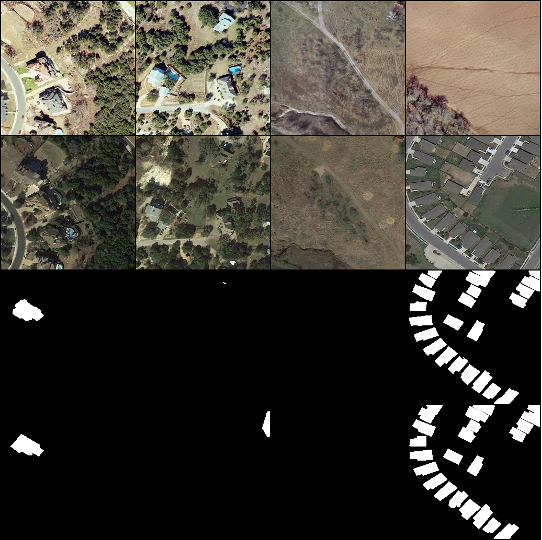
\includegraphics[width=\linewidth]{levir_attention_best.png}
        \caption{LEVIR-Attention}
    \end{subfigure}
    \begin{subfigure}[b]{0.3\linewidth}
        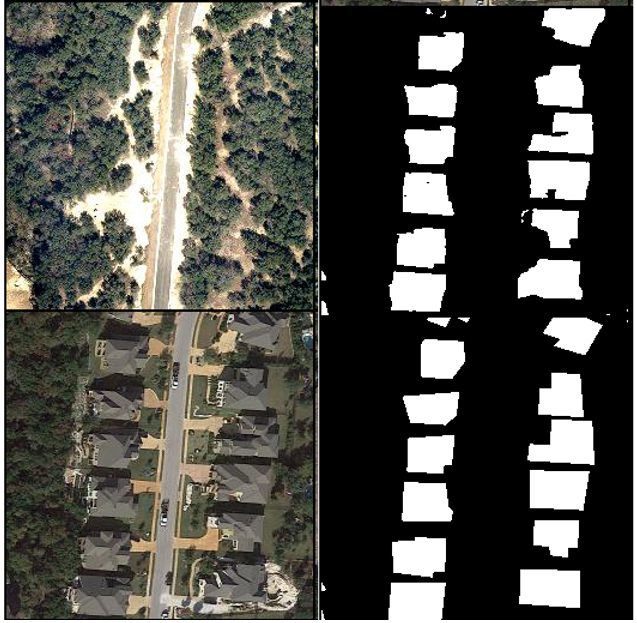
\includegraphics[width=\linewidth]{levir_fdaf_best.png}
        \caption{LEVIR-FDAF}
    \end{subfigure}
    \begin{subfigure}[b]{0.3\linewidth}
        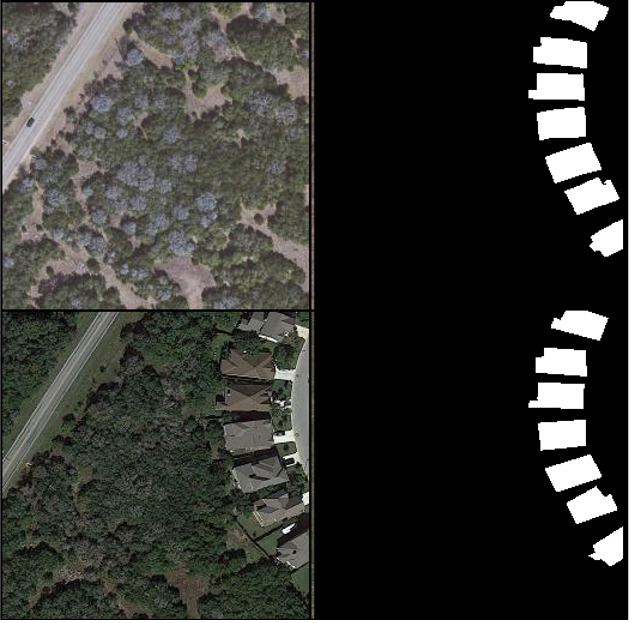
\includegraphics[width=\linewidth]{levir_attention_fdaf_best.png}
        \caption{LEVIR-Attention-FDAF}
    \end{subfigure}
    \begin{subfigure}[b]{0.3\linewidth}
        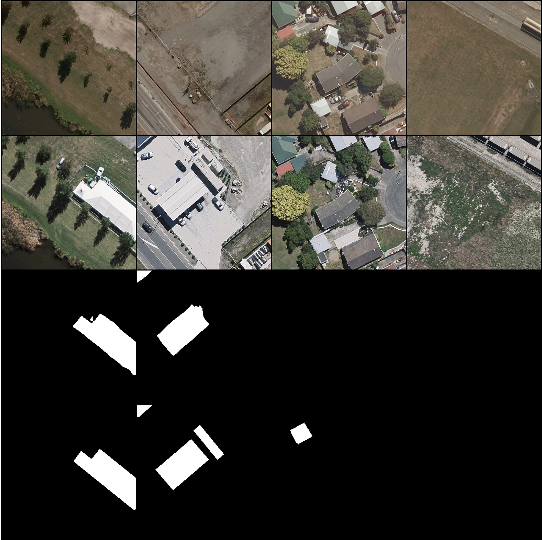
\includegraphics[width=\linewidth]{whu_attention_best.png}
        \caption{WHU-Attention}
    \end{subfigure}
    \begin{subfigure}[b]{0.3\linewidth}
        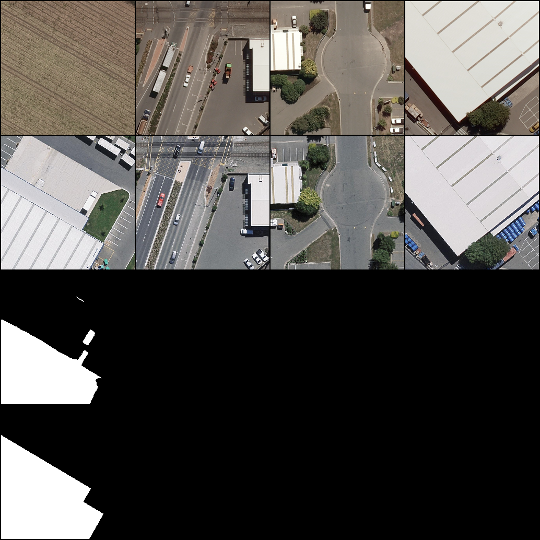
\includegraphics[width=\linewidth]{whu_fdaf_best.png}
        \caption{WHU-FDAF}
    \end{subfigure}
    \begin{subfigure}[b]{0.3\linewidth}
        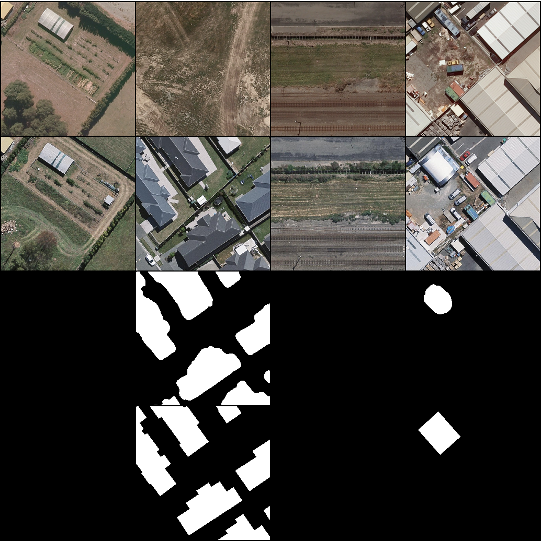
\includegraphics[width=\linewidth]{whu_attention_fdaf_best.png}
        \caption{WHU-Attention-FDAF}
    \end{subfigure}
    \caption{Qualitative results}
    \label{fig:qualitative_results}
\end{figure}

\subsection{Experimental Details}
One NVIDIA A6000 Ada Generation GPU was allocated and used for each experiment. As for the dataset, we cropped at 256x256 for both LEVIR-CD and WHU-CD, like baseline. In LEVIR, we used 7,120 train data and 2,048 validation data, and in WHU-CD, we used 5,952 train data and 1,488 validation data. The batch size was set to 8 during training, and Adam optimizer was used for the learning rate. In the case of LEVIR, it was learned for 120 epoch and in the case of WHU, 80 epoch, and the best validation score was recorded every epoch. 
\end{document}